\chapter{Menu File}
\minitoc  

\section{Open surface}
.stl, .ply, .vtk surfaces can be open via this menu. ISE-MeshTools does not manage textures associated with meshes; still, you can open .obj files, but associated textures will not be loaded. When opening a .ply file containing RGB colors (for instance a file painted manually or automatically with ``MeshLab") or a .vtk file containing RGB scalars, these colors are placed inside the ``RGB" scalars. MeshTools will reinitialize the ``RGB" scalars whenever you change the object's color or whenever you activate tag display mode or scalar display mode : if these colors are important to you, you may convert them to TAG values in the menu Tags$\rightarrow$Convert RGB colors to tags before changing the object color or display mode/before changing tags or any color scale activated.

\section{Save surface}
Selected surfaces can be saved into files. If no surface is selected, the following message appears:\\
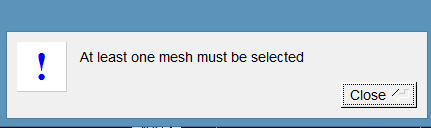
\includegraphics[scale=0.5]{images/File/Save_message.png}
If more than one mesh are selected, the following message shows up:\\
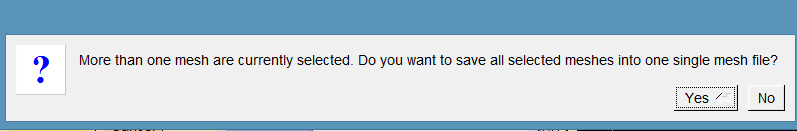
\includegraphics[scale=0.5]{images/File/Save_message2.png}

\subsection{Save .ply}

\begin{minipage}{0.5\textwidth}
Options:
\begin{itemize}
\item File type: you can save .ply data in binary (little or big endian)
or ASCII formats.
\item Position : you can keep object original coordinate system or
save the surface in its current position.
\item Normales : you can chose whether you wish to save normales.
\end{itemize}

\end{minipage}    
\begin{minipage}{0.5\textwidth}\centering
  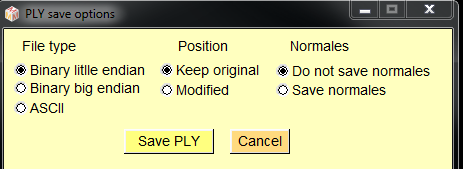
\includegraphics[scale=0.45]{images/File/Save_ply_new.png}
 \captionof{figure}{PLY save options window}
 \end{minipage} 

Note that the ``RGB" scalar (object rendering color, depending on which rendering mode you
are using) will be saved inside the .ply file. This means that Tag / Scalar / Object color can be exported and viewed in other software such as MeshLab.


\subsection{Save .stl}

\begin{minipage}{0.5\textwidth}
Options:
\begin{itemize}
\item File type: you can save .stl data in binary (little endian) or
ASCII formats.

\item Position : you can keep object original coordinate system or save the surface in its current position
\end{itemize}

\end{minipage}    
\begin{minipage}{0.5\textwidth}\centering
  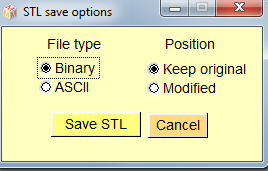
\includegraphics[scale=0.5]{images/File/Save_stl.png}
 \captionof{figure}{STL save options window}
 \end{minipage} 





\subsection{Save .vtk}
\begin{minipage}{0.5\textwidth}
Vtk mesh file format is by far not as widespread as stl or ply
format. However, it is extremely useful as it allows to store
scalar and tag values at each vertex or at each triangle.
Options:
\begin{itemize}
\item File type: you can save .vtk data in binary (little endian) or
ASCII formats.

\item Position : you can keep object original coordinate system
or save the surface in its current position
\end{itemize}
\end{minipage}    
\begin{minipage}{0.5\textwidth}\centering
  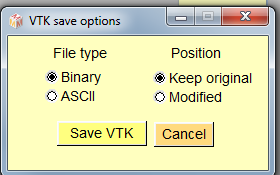
\includegraphics[scale=0.5]{images/File/Save_vtk.png}
 \captionof{figure}{VTK save options window}
 \end{minipage} 
\noindent
Note that the ``RGB" scalar (object rendering color, depending on which rendering mode you are
using) will be saved inside the .vtk file.
\subsection{Save .obj}

\begin{minipage}{0.5\textwidth}
ISE-MeshTools does not manage textures associated with
meshes. Still, you can save meshes in .obj format, but
textures will not be saved.
Options:
\begin{itemize}
\item Position : you can keep object original coordinate system
or save the surface in its current position
\end{itemize}
\end{minipage}    
\begin{minipage}{0.5\textwidth}\centering
  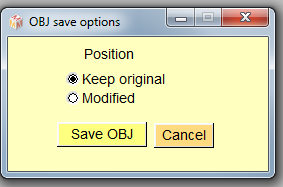
\includegraphics[scale=0.5]{images/File/Save_obj.png}
 \captionof{figure}{OBJ save options window}
 \end{minipage} 


\section{Position}
In ISE-MeshTools, mesh position consists in two
4*4 square matrices: one matrix is used as the
aspect matrix (by default the identity matrix),
and the other one as the position matrix. These
matrices can be opened and saved in ``.pos"
format (see Fig. \ref{position_file}).


\begin{figure}
  \centering
  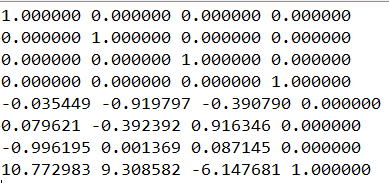
\includegraphics[scale=0.5]{images/File/Position_file.png}
 \caption{Example of .pos position file. The first 4 lines correspond
to the aspect matrix, and the 4 last lines to the position matrix.}
\label{position_file}
\end{figure}
 



\subsection{Load position}
If no surface is selected, the following message
appears:\\
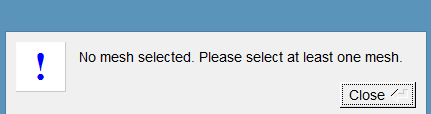
\includegraphics[scale=0.5]{images/File/open_position1.png}
\\
If more than one mesh are selected, the following message shows up :\\
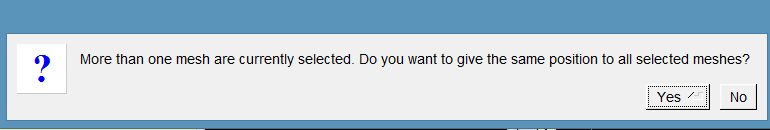
\includegraphics[scale=0.5]{images/File/open_position2.png}

\subsection{Load transposed position}
This option may be useful in the following case:
\begin{itemize}
\item Let us suppose that you did modify the position of a given surface and saved its position
\item Then you have saved the surface in its current modified position (that is : the original position of the
surface is lost).
\end{itemize}

For some reason, you may need to open the surface in its original position. To do so, you may apply this option (apply transposed position matrix to the modified surface).
Note : this option only works if the aspect matrix was not modified.

\subsection{Save position}
Mesh aspect and position matrices can be saved in ``.pos" format. If no surface is selected, the
following message appears:\\
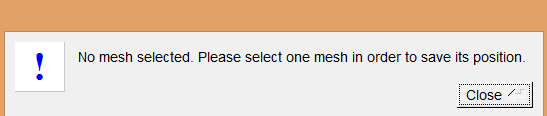
\includegraphics[scale=0.5]{images/File/save_pos1.png}
\\
If more than one mesh are selected, the following message shows up:\\
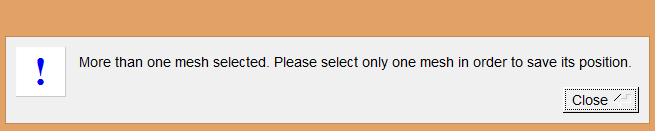
\includegraphics[scale=0.5]{images/File/save_pos2png.png}

\subsection{Edit manually aspect and position matrices}
There are two ways to access the object matrix editor :
\begin{itemize}

\item Either select one surface and click on ``
\includegraphics[scale=0.7]{images/pixmap/mat.png}"(edit first selected object position and aspect matrices).
\item Or select one surface and click on ``edit selected surfaces$\rightarrow$Rendering modifications$\rightarrow$ edit first
selected object position and aspect matrices".
\end{itemize}



This opens the ``Object Matrix" window, in which the aspect and position matrices can be edited. See ``Edit selected surfaces" section \ref{edit_mat_section} (Rendering modifications$\rightarrow$ edit first selected object position and aspect matrices) for further information.


\section{Project}
When working with multiple surface objects, 
loading surfaces and associated positions one
by one becomes fastidious. Besides, after having digitized landmarks, flags or having set tag names and colors, or having defined orientation labels, you may wish to open or save this information along with surface files. You may open and
save series of meshes and associated position matrices, landmarks, flags, tag colors and labels and orientation labels using this menu. ``Project" files (.ntw) files are organized the
following way (see Fig. \ref{project_file}):\\
- Optional: name of orientation label file (.ori)\\
- Optional: name of tag file (.tag)\\
- Optional: name of flag file (.flg)\\
- Optional: name of landmak file (.lmk, .ver, .stv or .cur)\\
- Name of surface 1 file\\
- Name of position 1 file associated to surface 1\\
- Surface 1 RGB color and transparency\\
- Name of surface 2 file\\
- Name of position 2 file associated to surface 2\\
- Surface 2 RGB color and transparency (etc...)\\
 
Surface files can be of the following types : .stl, .vtk, .ply and .obj\\
``.ntw" files can be constructed manually, providing that the refered surface and position files exist.



\begin{figure}
  \centering  
 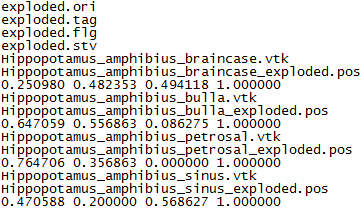
\includegraphics[scale=0.5]{images/File/Ntw.png}
 \captionof{figure}{Example of project .ntw file containing references to orientation labels, tags labels and colors, flags and landmarks files.}
\label{project_file}
\end{figure}

\subsection{Open project}
Loads a .ntw file

\subsection{Save project}
\begin{figure}
  \centering  
 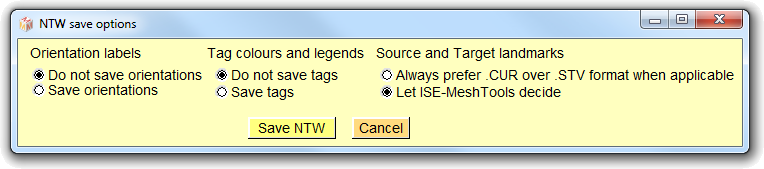
\includegraphics[scale=0.5]{images/File/Save_ntw.png}
 \captionof{figure}{Save project window.}
\label{save_project_file}
\end{figure}
The Save project window (\ref{save_project_file}) opens and asks whether :  
\begin{itemize}
\item orientation labels should be saved along with the project (by default, orientation labels are not saved, as orientation labels are quite rarely set by users). 
\item tag colors and legends should by saved (by default, .tag file are not saved along with the project, as tag setting is not the most common task). 
\item to prefer .CUR over .STV format when applicable or to let ISE-MeshTools decide which landmark file format is best when saving projects. We advise you to let ISE-MeshTools decide unless you are in the process of digitizing curves (for instance on inner ears). 
\end{itemize}
Furthermore, saving a .ntw file implies saving all selected surfaces. Though ISE-MeshTools can open .ntw files implicating .stl, .ply and .obj surfaces, when saving a .ntw project, surface files will be saved in .vtk format in order to keep potential tag / scalars associated to each saved surface. Each surface file will be given the name of the original file. Each position file will be given a name which starts with the name of the associated surface and ends with the name of the project. In the .ntw file example shown above, the surface files are 
\begin{itemize}
\item ``Hippopotamus\_amphibius\_braincase.vtk" 
\item ``Hippopotamus\_amphibius\_bulla.vtk" 
\item ``Hippopotamus\_amphibius\_petrosal.vtk" 
\item ``Hippopotamus\_amphibius\_sinus.vtk" 
\end{itemize}
\noindent and the project name is ``exploded.ntw". The advantage of naming position files that way is you may construct different .ntw files with different associated surface files using a same set of surfaces. Requirement : all selected surfaces saved via this option
need to have distinct names. Note : When working with ``project" files, you may need at
some point to rename some of the object surfaces. To do so, select one surface, click on 
\includegraphics[scale=0.7]{images/pixmap/name.png}: the ``Edit Name" window appears (see Fig. \ref{edit_object_name_window}).
Press ok to modify the name of that surface object. See tutorial ``working with projects" for further information.

\begin{figure}
  \centering  
 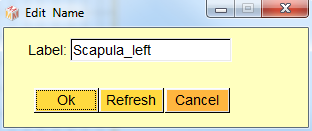
\includegraphics[scale=0.5]{images/Icons/edit_name.png}
 \captionof{figure}{Edit name window.}
\label{edit_object_name_window}
\end{figure}




\section{Landmarks}
As mentioned earlier, landmarks can be set on surfaces by pressing ``L" + left mouse click.\\

Two series ofconventional landmarks can be set : ``normal" and ``target" landmarks. As mentioned earlier, in the ``normal" landmark mode (button 
\includegraphics[scale=0.7]{images/pixmap/Landmarks4.png} active), pressing ``L" + left mouse click results in
the creation a ``normal" landmark (a red one). In the ``target" landmark mode (button 
\includegraphics[scale=0.7]{images/pixmap/Landmarks6.png} active),
pressing ``L" + left mouse click will create a ``target" landmark (a yellow one). ``Normal" and ``target" landmarks can be loaded and saved.\\
Selected ``normal"/"target" landmarks can be reordered using the following buttons. Pressing ``
\includegraphics[scale=0.7]{images/pixmap/s_dessous_17.png}"
will place the selected landmarks earlier in the ``normal"/"target" landmark list, while pressing ````
\includegraphics[scale=0.7]{images/pixmap/s_dessus_17.png}""
will place them one step further, respectively.\\\\
ISE-MeshTools can manage three types of landmark files: ``.LMK", ``.VER" and ``.STV" files.
\begin{itemize}
\item 
 .LMK files contain a series of lines, each line
being constructed the following way (see Fig. \ref{LMK_file}): landmark
name (without space or tab character),
landmark coordinates. Note that each landmark name does not need to be of the form ``landmark"+landmark number. Meanwhile, the name should not hold space or tab
characters.
\item .VER files contain a series
of lines, each line being
constructed the following
way (see Fig. \ref{VER_file}): landmark name (without space or tab character), landmark coordinates, landmark orientation.
\item .STV files may contain one or two series of line. The first line contains two integers, the first being the type of landmark (0 for ``normal" or 1 for ``target"), the second being the number of lines of landmarks of this type which are expected to follow, constructed the following way: landmark name (without space or tab character), landmark coordinates, landmark orientation. An example of .STV file containing both ``normal" and ``target" landmarks is given in Fig. \ref{STV_file}. Note that the number of ``normal" and ``target" landmarks saved within a .STV file can differ.
\end{itemize}
\begin{figure}
  \centering
  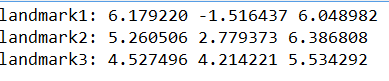
\includegraphics[scale=0.5]{images/Landmarks/LMK_file.png}
 \caption{Example of .LMK file}
\label{LMK_file}
\end{figure}

\begin{figure}
  \centering
  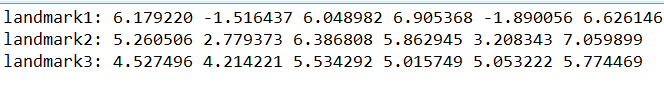
\includegraphics[scale=0.5]{images/Landmarks/VER_file.png}
 \caption{Example of .VER file}
\label{VER_file}
\end{figure}
\begin{figure}
  \centering
  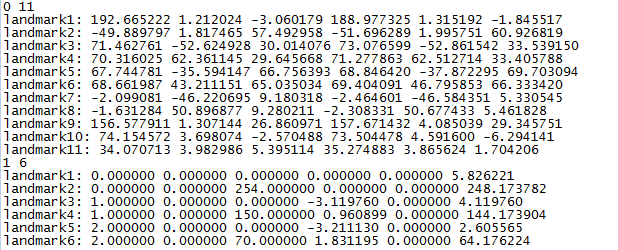
\includegraphics[scale=0.5]{images/Landmarks/STV_file.png}
 \caption{Example of .STV file}
\label{STV_file}
\end{figure}

\subsection{Load landmarks}
Landmarks opened using this option will be put in the ``normal" landmark list (red landmarks)
\subsection{Save landmarks}
You may decide whether you wish to save only selected ``normal" landmarks or all selected and
unselected ``normal" landmarks (the red ones).
\subsection{Save target landmarks}
You may decide whether you wish to save only selected ``target" landmarks or all selected and
unselected ``target" landmarks (the red ones).
The ``Landmarks" chapter (chapter \ref{landmark_chapter}) and the tutorial ``working with landmarks" contain further information regarding landmark digitization with ISE-MeshTools
\subsection{Load source and target landmarks}
Landmarks opened using this option will put in the ``normal" and/or ``target" landmark lists depending on how the .STV file is constructed.

\subsection{Save source and target landmarks}\label{STV_section}
All ``normal" and``target" landmarks will be saved inside the .STV file.

\section{Curves}\label{file_curve_section}
3D Curves are constructed in ISE-MeshTools using 2 series of landmarks : a series of ``normal"
landmarks, and a series of ``target" landmarks of equal sizes. ``Target" landmarks are referred to as
``curve handles", when they are used to construct curves (``Target" landmarks can also be used to
achieve TPS deformation, see later in this documentation). By default, curves are not drawn in the
main 3D window : curves start being drawn when the checkbox ``draw curves" is checked in the menu
``Viewing opt." (
\includegraphics[scale=0.7]{images/Landmarks/Draw_curves.png}). Curves are draw green when no landmark/curve handle belonging to
the curve is selected. Curves are drawn red when at least one landmark / curve handle involved in the
curve is selected. Two different cases are considered:
\begin{itemize}

\item Case 1: the numbers of ``normal" and ``handle/target" landmarks differ. In that case, a curve is a series of lines passing through ``normal" landmarks.
\item Case 2: the numbers of ``normal" and ``handle/target" landmarks differ. In that case, a curve is a
series of cubic Bezier curves passing through ``normal" landmarks. For a given set of 2 ``normal"
consecutive landmarks (Ln and Ln+1) and their associated curve ``handles" (Hn and Hn+1), a mirror
image of Hn+1 relative to Ln+1 (H'n+1) is constructed. The Bezier curve involving Ln, Ln+1, Hn and
Hn+1 starts from Ln, going toward Hn, and arrives at Ln+1 coming from the direction of H'n+1.

\end{itemize}


The explicit form of the curve is :
\begin{equation}
B(t) = (1-t)^{3}Ln + 3(1-t)^{3}tHn + 3(1-t)t^{2}H'n+1 +t^{3}Ln+1, t \in[0,1]
\end{equation}
In order to be able to digitize several curves using a given set of normal and target landmarks,
``normal" landmarks curves can be given 4 flags (see section \ref{landmarks_curves_section} ``Landmarks $\rightarrow$ Landmarks
involved into curves" for further details):\\
Flag ``0" : landmark is placed inside the curve (drawn ``red").\\
Flag ``1" : landmark is a curve start (drawn ``green").\\
Flag ``2" : landmark is placed inside the curve, and is a curve ``milestone" (drawn blue) .\\
Flag ``3" : landmark is placed inside the curve, and should be connected to the preceding curve
starting point. When landmark n is flagged that way, landmarkn+1 will be set as a curve starting point.\\
Flag ``2" is used to decompose a given curve into curve segments (see ``export curves as landmark file"). By default, a curve comprises 1 segment\\
Flag ``3" is used to close a curve (by default, curves are open).\\
3D curves are loaded and saved into .CUR files, which contain a series of lines, each line being
constructed the following way: name (without space or tab character), curve ``normal" landmark
coordinates, curve ``handle" coordinates, flag.
In the example shown below, 4 curves are defined :\\
- an open curve starting from landmark 1 and ending at landmark 7\\
- a closed curve involving landmarks 8 to 12\\
- a closed curve involving landmarks 13 to 20\\
- a closed curve involving landmarks 21 to 26\\
These four curves contain only one segment (no curve milestone was set within those 4 curves).
Note that each name does not need to be of the form ``landmark"+ number. Meanwhile, the name
should not hold space or tab characters.
\begin{figure}[t] 
  \centering
  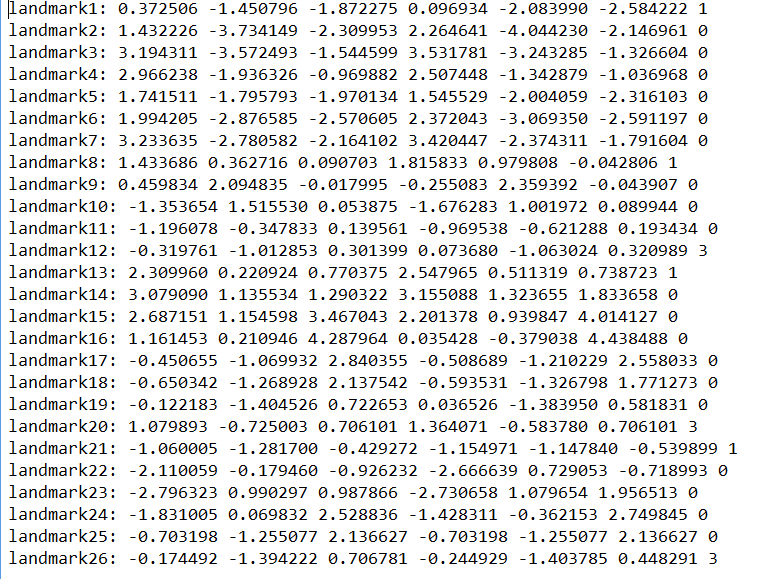
\includegraphics[scale=0.5]{images/Landmarks/CUR_file.png} 
	\caption{Example of .CUR file}
 
\end{figure}

\subsection{Load curves}
This menu allows the user to load a .CUR file.
\subsection{Save curves}
This menu allows the user to save current landmarks and curve handles as a .CUR file. This action is only allowed if the number of ``normal" landmarks and ``target" landmarks is the same. If not, the following message appears:\\
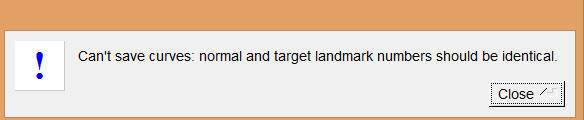
\includegraphics[scale=0.5]{images/Landmarks/Not_identical.png}
\\
If you are in the process of digitizing curves (and do not have achieved to digitize the same number of ``normal" and ``target"  landmarks and wish to save the current state of your work, you may decide to save a .STV file (see section \ref{STV_section}).


\subsection{Export curves as landmark file}
\begin{minipage}{0.55\textwidth}

Curves can be transformed in a series of equidistant
landmarks using this option. The curve decimation window
appears.
Each curve/curve segment is saved as a number of
equidistant landmarks. In the present example, each curve/
curve segment is saved as 20 equidistant landmarks.

\end{minipage}  
 \begin{minipage}{0.45\textwidth}\centering
  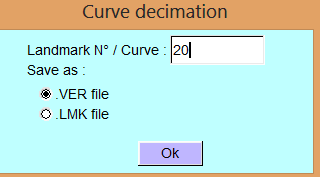
\includegraphics[scale=0.5]{images/Landmarks/Export_curves.png}
 \captionof{figure}{Curve decimation window}
 \end{minipage} 

When pressing ``Ok", if the numbers of ``normal" landmarks and ``target" landmarks differ, the
following message appears:\\
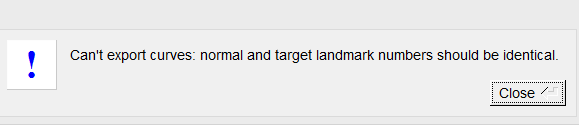
\includegraphics[scale=0.5]{images/Landmarks/Can_not_export.png}

\subsection{Save curve infos (length per curve ...)}
\begin{minipage}{0.55\textwidth}

Each curve /curve segment length can be saved as a .txt file
using this option.
The ``Landmarks" chapter (chapter \ref{landmark_chapter}) and the
tutorial ``Working with curves" contain further important
information regarding curve digitization with ISE-MeshTools.

\end{minipage}  
 \begin{minipage}{0.45\textwidth}\centering
  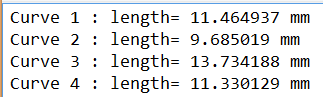
\includegraphics[scale=0.5]{images/Landmarks/Curve_infos.png}
 \captionof{figure}{Example of curve info file}
 \end{minipage} 



\section{Tags and flags}

\begin{minipage}{0.55\textwidth}
- Tag colors and names can be edited interactively by
clicking on 
\includegraphics[scale=0.7]{images/pixmap/Show_Tag_Window2.png}, which opens the tag window (see the chapter
``Tags" (chapter \ref{tags_chapter}) and the tutorial ``Working with tags" for
further information).\\
- By default, Tags are not visible. To activate/deactivate tag
display, click on 
\includegraphics[scale=0.7]{images/pixmap/Show_Tag_Window.png}\\
- Using ``Tag display mode" (
\includegraphics[scale=0.7]{images/pixmap/Tag_select_mode.png}) is useful when editing
surface tags.\\
25 Tag names and associated colors can be defined in ISEMeshTools.
Tag colors files (.TAG) consist of 25 pairs lines,
each pair being constructed following way :\\
line 2*n: Tag name\\
line 2*n+1: Tag color and transparency
\end{minipage}  
 \begin{minipage}{0.45\textwidth}\centering
  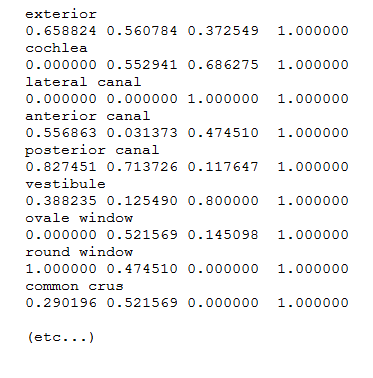
\includegraphics[scale=0.5]{images/Icons/Tags.png}
 \captionof{figure}{Example of .TAG file}
 \end{minipage} 

\noindent
\begin{minipage}{0.55\textwidth}
Regarding flags, as stated earlier, one series of ``flag landmarks" can be set in ISE-MeshTools (button 
\includegraphics[scale=0.7]{images/pixmap/Flag01.png} should
be pressed). To edit flag label, length and color, select one
flag landmark, click on 
\includegraphics[scale=0.7]{images/pixmap/Flag02.png}. The ``edit flag" window appears.
Pressing ok will update the label, the color and the
length associated to the selected flag, which in turn will be
unselected. If you wish to edit a second flag, select it and press ``Refresh". The current color, length
and label of the newly selected flag will appear in the edit flag window.
\end{minipage}  
 \begin{minipage}{0.45\textwidth}\centering
  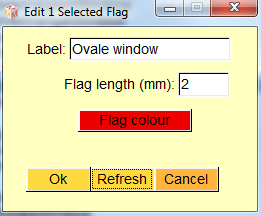
\includegraphics[scale=0.5]{images/Flags/Edit1flag.png}
 \captionof{figure}{Edit Flag window}
 \end{minipage} 
\noindent
Flags are saved using the .FLG file format, which consists of n pairs of lines constructed the following way :\\
line 2*n: Flag name\\
line 2*n+1: Flag coordinates, flag orientation, flag length and color.

\subsection{Load tag colors and labels}
Select a .TAG file using this menu $\rightarrow$ Then open the tag window (
\includegraphics[scale=0.7]{images/pixmap/Show_Tag_Window2.png}) : Tag labels, colors and
transparencies should have been updated.
\subsection{Save tag colors and labels}
This option saves the current state of tag labels, colors and transparencies in a .TAG file.

\subsection{Load flags}
Select a .FLG file using this menu

\subsection{Save flags}
This option saves the current flag landmarks into a .FLG file, regardless their selection status.

\section{Save infos (surface area, volume...)}
\noindent
\begin{minipage}{0.55\textwidth}

Surface area, volume, triangle number and
vertex number of selected surface objects can be
saved in a .txt file using this option.
\end{minipage}  
 \begin{minipage}{0.45\textwidth}\centering
  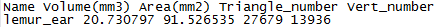
\includegraphics[scale=0.4]{images/File/Infos.png}
 \captionof{figure}{Example of info file}
 \end{minipage} 
\noindent

Note: surface objects should be closed in order to provide a correct estimation of object volume.
\section{Orientation labels}
The coordinate system orientation helper labels can be saved into ``.ORI" files, which are .txt files
containing 6 lines, 1 for each axis.


\subsection{Load orientation labels}
Select a .ORI file using this menu $\rightarrow$ Then open the orientation labels window window (Viewing opt;
Orientation labels) : the 6 orientation labels should have been updated.

\subsection{Save orientation labels}
This option saves the current state of orientation labels in a .ORI file.

